
%(BEGIN_QUESTION)
% Copyright 2008, Tony R. Kuphaldt, released under the Creative Commons Attribution License (v 1.0)
% This means you may do almost anything with this work of mine, so long as you give me proper credit

Sketch a circuit whereby this loop-powered pressure transmitter sends a signal to an analog current meter (acting as a remote pressure gauge).  Include any necessary power sources in your completed circuit:

\vskip 50pt

$$\includegraphics[width=15.5cm]{i03202x01.eps}$$

\vfil 

\underbar{file i03202}
\eject
%(END_QUESTION)





%(BEGIN_ANSWER)

This is a graded question -- no answers or hints given!

%(END_ANSWER)





%(BEGIN_NOTES)

This is just one possible solution:

$$\includegraphics[width=15.5cm]{i03202x02.eps}$$

\vskip 10pt

Alternative solution:

$$\includegraphics[width=15.5cm]{i03202x03.eps}$$

\vskip 10pt

\filbreak

A good problem-solving technique to apply here is sketching arrows showing where conventional flow (current) enters and exits each component, based on its voltage polarity and its identity as either a source or a load.  Once these arrows are sketched, it becomes a trivial matter to connect tip-to-tail to form a series circuit:

$$\includegraphics[width=15.5cm]{i03202x04.eps}$$

{\it Any} connections that put the tip of one arrow connecting the tail of another will form a valid series circuit!

%INDEX% Pictorial circuit review (4-20 mA loop)

%(END_NOTES)


